\documentclass[conference]{IEEEtran}

\usepackage{amsmath}
\usepackage{graphicx}
\usepackage{subfig}
\usepackage{paralist}
\usepackage{tikz}
\usepackage[normalem]{ulem}

\providecommand{\e}[1]{\ensuremath{\times 10^{#1}}}

% correct bad hyphenation here
\hyphenation{op-tical net-works semi-conduc-tor}

\begin{document}

\title{Predicting Reciprocity in Social Networks}

\author{\IEEEauthorblockN{Anonymous}
\IEEEauthorblockA{Anonymous Department\\
Anonymous Institution \\
Anonymous Location \\
anon@whoare.you}
\and
\IEEEauthorblockN{Anonymous}
\IEEEauthorblockA{Anonymous Department\\
Anonymous Institution \\
Anonymous Location \\
anon@whoare.you}
\and
\IEEEauthorblockN{Anonymous}
\IEEEauthorblockA{Anonymous Department\\
Anonymous Institution \\
Anonymous Location \\
anon@whoare.you}}

% make the title area
\maketitle

\begin{abstract}
%\boldmath
In this paper we investigate methods of predicting reciprocity in social networks, and use decision trees and regression models to determine good indicators of reciprocity. 
We extract a network based on directed @-messages sent between users in Twitter, and discover that the ratio of a node's outdegree to its indegree is the best predictor of reciprocity.  
Moreover, we find that heuristics used in link prediction do not necessarily perform well in reciprocity prediction. 
In fact, using only simple properties that relate to the degree of a node or the number of messages that it sends or receives is sufficient in obtaining maximum accuracy in this prediction <<rephrase?>>.
\end{abstract}

% no keywords

% For peer review papers, you can put extra information on the cover
% page as needed:
% \ifCLASSOPTIONpeerreview
% \begin{center} \bfseries EDICS Category: 3-BBND \end{center}
% \fi
%
% For peerreview papers, this IEEEtran command inserts a page break and
% creates the second title. It will be ignored for other modes.
\IEEEpeerreviewmaketitle

\section{Introduction}
Reciprocity prediction and link prediction are inherently different problems --- while the link prediction task is about predicting the occurrence of rare events, reciprocity prediction estimates the ``balance'' of a relationship.

\subsection{Related work}
Tyler and Tang~\cite{TylerTang} showed that reciprocity 
To be written.

\subsection{Twitter as a domain to analyze}
Twitter is a good domain to explore the superposition of the reciprocated and unreciprocated networks. 
The reciprocated network consists of mainly mutual interactions between friends or people in the same social circle, while the unreciprocated network consists of interactions between individuals in different social circles. 
We can also relate these types of interactions to the concept of status - where people with similar status participate in reciprocal interactions (e.g. messages between friends), while those with dissimilar status participate in unreciprocated interactions (e.g. messages from fans to celebrities).

\subsection{Problem definition}
We are generally interested in determining whether a relationship is reciprocated.
The input to our prediction problem is a directed graph $G=(V,E)$ and a node pair $\{v,w\}$, where $v,w \in V$ but all edges between $v$ and $w$ removed. 
Our task is to predict the direction of edges between $v$ and $w$, and we see that the problem of predicting reciprocation can be defined in two ways. 
First, we consider the formulation in which we decide whether a $\{v,w\}$ relationship is symmetric (that is, both $(v,w)$ and $(w,v)$ exist) or is asymmetric (only one of the directed $(v,w)$, $(w,v)$ relationship exists).
We make this prediction under the assumption that at least one directed edge exists between $v$ and $w$. 
In the second formulation, we ask whether $(w,v)$ exists given that there is the $(v,w)$ edge. 
It would appear that predicting a symmetric relationship between nodes is a more difficult task than predicting reciprocation in a specific direction, and we show that this is indeed the case.

\subsection{Notation}
The number of messages users author in Twitter exhibits a long-tail distribution; many users produce only a small number of messages.
In this work, we will focus on users who have produced a large number of @-messages.
We consider the subgraphs of the form $G_n = (V_n, E_n)$, where $V_n = \{v~|~v \in V, v \text{ sent } \ge n \text{ messages}\}$ and $E_n = \{e=(v,w)~|~e \in E,~v \text{ and } w \in V_n\}$.
This subgraph captures the @-messaging interactions between users who are prolific Twitter users.
We use the notation $v \xrightarrow{k} w$ to indicate that $v$ sent at least $k$ @-messages to $w$. 
From this definition we can formalize reciprocity in terms of $k$. 
We say that an edge $(v,w)$ is reciprocated if both $v \xrightarrow{k} w$ and $w \xrightarrow{k} v$, and unreciprocated if only $v \xrightarrow{k} w$.
Let the set of reciprocated edges be \(E_k^r = \{ (v,w) : v \xrightarrow{k} w \text{ and } w \xrightarrow{k} v \} \), and the set of unreciprocated edges be \(E_k^u = \{ (v,w) : v \xrightarrow{k} w\}\).
Finally, let $\deg^-(v)$ and $\deg^+(v)$ respectively denote the indegree and outdegree of node $v$, $\operatorname{msg}^-(v)$ and $\operatorname{msg}^+(v)$ be the messages received and sent by $v$, and $\Gamma^-(v) = \{w| (w,v) \in E\}$ be set of people who send messages to $v$.

\section{Dataset description}
% TODO: Cite our other paper here for details about the data collection
We extract the \emph{@-message graph} from a large crawl of Twitter that took place between August 2009 and January 2010.
More than three-billion messages from over 60 million users were collected.  
The @-message graph is constructed by looking at Tweets a user $v$ authors which mention user $w$ at the beginning of the Tweet.  
The graph $G = (V,E)$ of users who authored at least one @-message contains 12,795,683 unique users who sent a total of 819,305,776 @-messages, with 156,868,257 unique directed interactions. 

We focus our analysis on the subgraph $G_{1000}$, the subgraph induced by users who authored at least 1000 @-messages. 
Furthermore, we only consider an edge $(v,w)$ to be present if at least 10 @-messages were sent from $v$ to $w$ (in our notation, $v \xrightarrow{10} w$).
In $G_{1000}$, we find that $|E^r_{10}| = 797,342$, $|E^u_{10}| = 349,258$.
HOW MANY USERS WAS THIS?

\section{Methods for Reciprocity Prediction}
Intuitively, features can measure whether $v$ and $w$ have similar status or a similar social circle, and both are potentially useful in predicting reciprocation. 
This section presents a survey of various methods that can be used in predicting reciprocity in networks. 
Each method assigns a value $\operatorname{val}(v,w)$ to a node pair $(v,w)$, or a value $\operatorname{val}(v)$ to a single node $v$. 
Given values corresponding to all node pairs (or nodes) in question, we can then choose threshold values or ranges where we predict reciprocity, and none otherwise.

For each property, we picked a single value $\operatorname{val}_{OPT}$ for which we predict every pair with value lower than $\operatorname{val}_{OPT}$ as unreciprocated and reciprocated otherwise, or vice versa, to maximize prediction accuracy. 
Intuitively, we expect that larger values of each property correspond to a stronger indication of reciprocity. 
For example, a high mutual neighbor count for the nodes $v$ and $w$ could strongly indicate the existence of a reciprocated link between them.

Now, given the two ways that we can formulate the prediction problem, we present four different mechanisms that we can use to predict reciprocity. 
The first attempts to answer the question of symmetry, while the other three answer the problem of reciprocity, with different limits on the amount of information about the nodes in question used.

\begin{enumerate}
\item SYM (predicting symmetry), where we predict whether an edge is bidirectional or asymmetric after removing all information about the edge in question but using existing information about $v$ and $w$, 
\item REV (predicting a reverse edge), where we predict whether a reverse edge exists given that the forward edge $(v,w)$ exists using information about $v$ and $w$, and finally 
\item REV-$w$ (predicting a reverse edge using only $w$), where we predict whether a reverse edge exists given that $(v,w)$ exists, but only using information about $w$ in making that prediction.
\item REV-$v$ (predicting a reverse edge using only $v$), where we predict whether a reverse edge exists given that $(v,w)$ exists, but only using information about $v$ in making that prediction.
\end{enumerate}

With this framework, we can now choose specific features of the @ message graph that we can plug in and compare their relative performance, and also their combined performance.

\subsection{Degree and message features}
It seems intuitive that the relative indegree or outdegree of nodes would indicate whether a pair of nodes are in a one-sided or two-sided relationship. 
If both have a similar indegree, this might indicate that they are at a similar social status in the network. 
In contrast, a disproportionate indegree would indicate that one user is a celebrity and the other is a non-celebrity, making it unlikely that their relationship is reciprocal.

For these features, we also looked at their absolute ``counterparts'', such as the outdegree of $v$ or the indegree of $w$ in the edge $(v,w)$):

\emph{Indegree and outdegree ratio} both measure the ratio of outdegrees or indegrees of two nodes, and we define $\operatorname{val}(v,w) = \deg^-(v)/\deg^-(w)$ or $\deg^+(v)/\deg^+(w)$, respectively.

\emph{Incoming message and outgoing message ratio} are similar, but instead uses the total number of messages that a node receives or sends, regardless of the nodes to which messages are sent or from which  messages are received. TODO: put the def here to be precise.

\emph{Incoming message/indegree ratio and outgoing message/outdegree ratio} compares the ratio of two nodes' incoming message to indegree ratio or outgoing message to outdegree ratio. 
A high incoming message to indegree ratio might characterize users who have a small group of friends with which they exchange many messages.
Alternatively, a low incoming message to indegree ratio could characterize highly connected (and thus high-status [do we want to make a status claim?]) people in a network, since the messages they receive are distributed over many more users.

\emph{Outdegree/indegree ratio} is a heuristic that characterizes the messaging activity of a single node.  
A large outdegree/indegree ratio might indicate a user of celebrity status because she receives many messages from many followers [make sure followers is mentioned somewhere earlier in the paper] but sends relatively few messages. 
Given a pair of nodes, we can compute the outdegree/indegree ratio as $\operatorname{val}(v,w) = \frac{\deg^+(v)}{\deg^-(v)} / \frac{\deg^+(w)}{\deg^-(w)}$.

\subsection{Link prediction features}
It is not intuitive whether methods that work well for link prediction would work well in predicting reciprocity. 
While link prediction asks whether an edge could exist between two nodes, reciprocity prediction asks whether a known directed-edge is actually bidirectional.
The following are some measures used in the link-prediction task:

\emph{Mutual neighbors} calculates the number of people to whom both $v$ and $w$ send messages ($|\Gamma^+(v) \cap \Gamma^+(w)|$), or the number of people from whom both $v$ and $w$ receive messages ($|\Gamma^-(v) \cap \Gamma^-(w)|$).

\emph{Jaccard's coefficient} is also based on the concept of mutual neighbors, calculates the similarity between two sets by taking the ratio of the cardinality of their intersection and their union: \[\operatorname{val}(v,w) = \frac{|\Gamma^-(v) \cap \Gamma^-(w)|}{|\Gamma^-(v) \cup \Gamma^-(w)|}.\]

\emph{Adamic and Adar} \cite{Adamic:2003ud} defined the similarity between web sites $v,w$ to be $ \sum_{\{x|v,w \text{ share feature }x\}} \frac{1}{\log{\text{frequency}(x)}} $, and we similarly define $\operatorname{val}(v,w)$ to be \[ \sum_{\{x|x \in \Gamma^-(v) \cap \Gamma^-(w)\}} \frac{1}{\log{\deg^-(x)}} .\]

\emph{Preferential attachment} is another popular heuristic in modeling network growth, where the probability that an edge forms with a specific node is proportional to its existing indegree. 
Here, $\operatorname{val}(v,w) = \deg^-(v)\cdot \deg^+(w)$, or $\deg^+(v)\cdot \deg^-(w)$. 
Notice that taking the ratio of these two values is equivalent to the outdegree/indegree ratio between two nodes.

\emph{Two-step paths (ratio)} is a simplification of Katz's \cite{Katz:1953un} measure of status by calculating the number of paths between two nodes. 
In this work, we only consider paths of length 2, and define $\operatorname{val}(v,w) = \operatorname{paths}^2(v,w)|$, where $\operatorname{paths}^2(v,w)$ is the set of paths from $v$ to $w$ of length $2$. 
The two-step paths ratio is simply the ratio of number of two-step paths from $v$ to $w$ to that from $w$ to $v$. 

TODO I can also calculate that in the case where you predict a reverse edge, you use the path from $v$ to $w$ in your calculation, thus adding a single on-step path to the calculation. 
But this ends up being worse, so probably it's not important to include.

\subsection{Different sets of features}
We examine several additional features, and for convenience, we further break these down into four sets of features:
\begin{enumerate}
	\item Absolute degree/message features - degree, messages, message-degrees, outdegree-indegrees
	\item Relative degree/message features - degree ratios, message ratios, message-degree ratios, and outdegree-indegree ratios
	\item Two-step hop features - mutual neighbors (in and out), and two step paths ($v$ to $w$ and $w$ to $v$)
	\item Link prediction features - all other link prediction features not mentioned
\end{enumerate}

\subsection{Two-step hops}
\begin{figure}[!t]
\centering
\caption{Two-step hops}
\label{fig_2step}
\subfloat[2-step ($v$ to $w$)]{
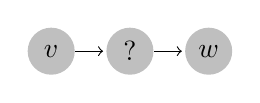
\begin{tikzpicture}[shorten >=1pt,->]
  \tikzstyle{vertex}=[circle,fill=black!25,minimum size=17pt,inner sep=0pt]

  \foreach \name/\x in {v/1, ?/2, w/3}
    \node[vertex] (G-\name) at (\x,0) {$\name$};

  \foreach \from/\to in {v/?, ?/w}
    \draw (G-\from) -- (G-\to);

\end{tikzpicture}}\quad
\subfloat[2-step ($w$ to $v$)]{
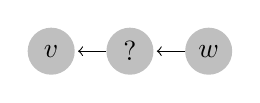
\begin{tikzpicture}[shorten >=1pt,->]
  \tikzstyle{vertex}=[circle,fill=black!25,minimum size=17pt,inner sep=0pt]

  \foreach \name/\x in {v/1, ?/2, w/3}
    \node[vertex] (G-\name) at (\x,0) {$\name$};

  \foreach \from/\to in {w/?, ?/v}
    \draw (G-\from) -- (G-\to);

\end{tikzpicture}}
\\
\subfloat[Mutual (in)]{
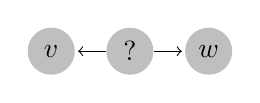
\begin{tikzpicture}[shorten >=1pt,->]
  \tikzstyle{vertex}=[circle,fill=black!25,minimum size=17pt,inner sep=0pt]

  \foreach \name/\x in {v/1, ?/2, w/3}
    \node[vertex] (G-\name) at (\x,0) {$\name$};

  \foreach \from/\to in {?/w, ?/v}
    \draw (G-\from) -- (G-\to);

\end{tikzpicture}}\quad
\subfloat[Mutual (out)]{
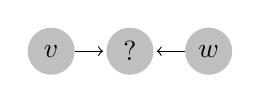
\begin{tikzpicture}[shorten >=1pt,->]
  \tikzstyle{vertex}=[circle,fill=black!25,minimum size=17pt,inner sep=0pt]

  \foreach \name/\x in {v/1, ?/2, w/3}
    \node[vertex] (G-\name) at (\x,0) {$\name$};

  \foreach \from/\to in {w/?, v/?}
    \draw (G-\from) -- (G-\to);

\end{tikzpicture}}
\end{figure}
The importance of ``friends of friends,'' or people two links away from a given node, lends itself to exploring features that directly arise out of the directed @-message graph. 
There are essentially four types of two-step hops, as shown in figure \ref{fig_2step}, corresponding to either the number of common in-neighbors or out-neighbors (mutual neighbors), or the number of directed paths from $v$ to $w$ or from $w$ to $v$ (two-step paths). 

If both $v$ and $w$ send messages to many common people, it is likely that they are in the same social circle, or it could be that $v$ and $w$ simply message the same celebrities. 
If $v$ and $w$ receive many messages from the same group of people, it could be that both $v$ and $w$ are in the same community, or that both $v$ and $w$ are celebrities (who may or may not talk to each other) and there is an overlapping fanbase.

As the number of paths from $v$ to $w$ increases, there are two conflicting forces of $w$ being popular and thus it unlikely for $w$ to reciprocate an edge from $v$ to $w$. 
The reverse case is simpler--- intuitively, as the number of paths from $w$ to $v$ increases, the likelihood that $w$ knows $v$ grows.

\begin{table}[!t]
\renewcommand{\arraystretch}{1.3}
\caption{Reciprocity Prediction Features}
\label{table_recmethods}
\centering
\begin{tabular}{|c||c|}
\hline
\bf{Feature} & $\mathbf{val}(v)$ or $\mathbf{val}(v,w)$\\
\hline
\multicolumn{2}{|c|}{\emph{Absolute degree/message features}} \\
\hline
Indegree or outdegree & $\deg^-(v)$ or $\deg^+(v)$ \\
Incoming or outgoing messages & $\operatorname{msg}^-(v)$ or $\operatorname{msg}^+(v)$ \\
Message-degree (in or out) & $\frac{\operatorname{msg}^-(v)}{\deg^-(v)}$ or $\frac{\operatorname{msg}^+(v)}{\deg^+(v)}$ \\
Outdegree-indegree & $\frac{\deg^+(v)}{\deg^-(v)}$ \\
\hline
\multicolumn{2}{|c|}{\emph{Relative degree/message features}} \\
\hline
Indegree ratio & $\deg^-(v) / \deg^-(w)$ \\
Outdegree ratio & $\deg^+(v) / \deg^+(w)$ \\
\hline
Incoming message ratio & $\operatorname{msg}^-(v) / \operatorname{msg}^-(w)$ \\
Outgoing message ratio & $\operatorname{msg}^+(v) / \operatorname{msg}^+(w)$ \\
\hline
Message-degree ratio (in) & $\frac{\operatorname{msg}^-(v)}{\deg^-(v)} / \frac{\operatorname{msg}^-(w)}{\deg^-(w)}$ \\
Message-degree ratio (out) & $\frac{\operatorname{msg}^+(v)}{\deg^+(v)} / \frac{\operatorname{msg}^+(w)}{\deg^+(w)}$ \\
\hline
Outdegree-indegree ratio & $\frac{\deg^+(v)}{\deg^-(v)} / \frac{\deg^+(w)}{\deg^-(w)} $ \\
\hline
\multicolumn{2}{|c|}{\emph{Link prediction features}} \\
\hline
Mutual neighbors (in) & $|\Gamma^-(v) \cap \Gamma^-(w)|$ \\
Mutual neighbors (out) & $|\Gamma^+(v) \cap \Gamma^+(w)|$ \\
\hline
Jaccard's coefficient (in) & $\frac{|\Gamma^-(v) \cap \Gamma^-(w)|}{|\Gamma^-(v) \cup \Gamma^-(w)}$ \\
Jaccard's coefficient (out) & $\frac{|\Gamma^+(v) \cap \Gamma^+(w)|}{|\Gamma^+(v) \cup \Gamma^+(w)}$ \\
\hline
Adamic/Adar & $\sum_{\{x|x \in \Gamma^-(v) \cap \Gamma^-(w)\}} \frac{1}{\log{\deg^-(x)}}$ \\
\hline
Preferential attachment ($v$ to $w$) & $\deg^+(v)\cdot \deg^-(w)$ \\
Preferential Attachment ($w$ to $v$) & $\deg^+(w)\cdot \deg^-(v)$ \\
\hline
Two-step paths ($v$ to $w$) & $ |\operatorname{paths}^2(v,w)|$ \\
Two-step paths ($w$ to $v$) & $ |\operatorname{paths}^2(w,v)|$ \\
\hline
Two-step paths ratio & $\frac{|\operatorname{paths}^2(v,w)|}{|\operatorname{paths}^2(w,v)|}$ \\
% $\frac{\sum_{i=1}^2 \beta^i|\operatorname{paths}^i(v,w)|}{\sum_{i=1}^2 \beta^i|\operatorname{paths}^i(w,v)|}$ Did badly
\hline
\end{tabular}
\end{table}

\section{Results and Discussion}

\subsection{Individual properties}
To calculate the accuracy of the individual heuristics, we calculated $\operatorname{val}$ for each feature on the subset $E_{10}^r \cup E_{10}^u$ of the graph $G_{1000}$, where equal numbers of edges were taken from the two sets of reciprocated and unreciprocated edges. 
This would give a baseline accuracy is 0.500, and you would achieve this by predicting that all edges were of one type. 
We applied the SYM and REV mechanisms to feature sets 2-4, and REV-$v$ and REV-$w$ to feature set 1.

We then picked a threshold value $\operatorname{val}_{OPT}$ to optimize prediction accuracy - we predicted reciprocity above the threshold, and non-reciprocity below (or vice versa depending on which performed better). 
Tables \ref{table_recresults_indiv} and \ref{table_recresults_indivVW} summarize the performance of each heuristic on the subgraph $G_{1000}, k=10$, while table \ref{table_recresults_indeg} summarizes the different mechanisms of prediction for a single heuristic.

In tables \ref{table_recresults_indiv} and \ref{table_recresults_indivVW}, a star ($*$) indicates that reciprocity was predicted when $\operatorname{val}$ was below the threshold, and a lack thereof indicates reciprocity was predicted when $\operatorname{val}$ was above the threshold.

In table \ref{table_recresults_indeg}, SYM$^+$ refers to the prediction mechanism where we aim to predict symmetry and predict all edges with values \emph{above} $val_{OPT}$ to be reciprocated, and REV$^-$ refers to the mechanism where we aim to predict whether a reverse edge $(w,v)$ exists given $(v,w)$ and predict all edges with values \emph{below} $val_{OPT}$ to be reciprocated. 

\subsubsection{Comparison of prediction mechanisms}
We observe higher accuracy for the REV task than SYM, as REV is ``easier" than SYM since you know more information about the edge $(v,w)$.

Comparing REV-$v$ to REV-$w$, we see REV-$w$ obtains higher accuracy compared to REV-$v$, and this is because we're trying to predict the existence of the edge from $w$ to $v$ given $(v,w)$, and knowing about $w$ is a lot more valuable than knowing about $v$.

Note that SYM$^-$, REV$^-$, REV$-w^+$ and REV-$v^-$ are such poor predictors that simply predicting that everything was reciprocated (or unreciprocated) would have been better.

\subsubsection{Comparison of methods of prediction}

\paragraph{Trends}
On the whole, outdegree-indegree ratio and the two-step paths ratio are the best indicators of reciprocity. 
In fact, outdegree-indegree ratio alone already achieves accuracy to within $\pm 5\%$ of a decision tree using every feature.

\paragraph{Sending and receiving}
When we look at features using one of the four mechanisms, the larger the value, the more likely it is for reciprocation to occur, and this is the case for a majority of features. 
For example, the \emph{larger} the indegree ratio, the more in-links $v$ has in relation to $w$, increasing the probability that $w$ will link to $v$, given that we know that $v$ already links to $w$.

However, the \emph{smaller} the outdegree-indegree ratio, the more likely reciprocation occurs. 
In other words, a small numerator and a large denominator in $\frac{\deg^+(v)}{\deg^-(v)} / \frac{\deg^+(w)}{\deg^-(w)} = \frac{\deg^+(v)\deg^-(w)}{\deg^-(v)\deg^+(w)}$ is a good indicator of reciprocation. 
And indeed, a large denominator indicates that $v$ has many in-links and $w$ has many out-links, both of which increase the probability that $w$ links to $v$.

Interestingly, separating the numerator and denominator from the outdegree-indegree ratio above, which corresponds to our two preferential attachment features, results in two very different results. 
While a small numerator does decently well (preferential attachment ($v$ to $w$)), a large denominator does not (preferential attachment ($w$ to $v$)) and this only performs marginally better than chance. <<TODO Why?>>

\paragraph{REV-$v$ vs. REV-$w$}
Not surprisingly, REV-$w$ performs better than REV-$v$ on almost all features, and where REV-$v$ performs better, the difference is not as significant [be more specific about significance?]. 
Analogous to whether you would want to know more about the features of a marketer ($v$) vs. a subscriber ($w$), knowing about the subscriber tells us more about the relationship between both. <<Expand>>

\begin{table}[!t]
\renewcommand{\arraystretch}{1.3}
\caption{Indegree performance - different methods}
\label{table_recresults_indeg}
\centering
\begin{tabular}{|c||c|c|}
\hline
\bf{Mechanism} & $\mathbf{val}_{OPT}$ (Percentile) & \bf{Accuracy} \\
\hline
\multicolumn{3}{|c|}{\emph{Indegree ratio}} \\
\hline
SYM$^+$ & 0.256 (40) & 0.702 \\
SYM$^-$ & - & - \\
REV$^+$ & 0.414 (46) & 0.759 \\
REV$^-$ & - & - \\
\hline
\multicolumn{3}{|c|}{\emph{Indegree of $v$ or $w$}} \\
\hline
REV-$w^+$ & - & - \\
REV-$w^-$ & 74 (61) & 0.731 \\
REV-$v^+$ &  61 (60) & 0.582 \\
REV-$v^-$ & - & - \\
\hline
\end{tabular}
\end{table}

\begin{table}[!t]
\renewcommand{\arraystretch}{1.3}
\caption{Reciprocity Prediction Method Performance: Individual (REV)}
\label{table_recresults_indiv}
\centering
\begin{tabular}{|c||c|c|}
\hline
\bf{Method} & $\mathbf{val}_{OPT}$ (Percentile) & \bf{Accuracy} \\
\hline
Indegree ratio & 0.414 (46) & 0.759 \\
Outdegree ratio & 0.667 (43) & 0.628 \\
\hline
Incoming message ratio & 0.333 (48) & 0.772 \\
Outgoing message ratio & 0.905 (46) & 0.547 \\
\hline
Incoming message-indegree ratio & 0.650 (39) & 0.569 \\
Outgoing message-outdegree ratio & 0.791 (33) & 0.615* \\
\hline
Outdegree-indegree ratio & 1.72 (53) & 0.820* \\
\hline
Mutual neighbors (in) & 10 (61) & 0.552 \\
Mutual neighbors (out) & 8 (51) & 0.580 \\
\hline
Jaccard's coefficient (in) & 0.0345 (48) & 0.684 \\
Jaccard's coefficient (out) & 0.0637 (55) & 0.660 \\
\hline
Adamic/Adar & 1.94 (55) & 0.561 \\
\hline
Two-step paths ($v$ to $w$) & 6 (59) & 0.517* \\
Two-step paths ($w$ to $v$) & 5 (51) & 0.657 \\
Two-step paths ratio & 0.556 (52) & 0.760 \\
% Two-step paths ratio (undirected) & 0.259 (34) & 0.516 \\
\hline
Preferential attachment ($v$ to $w$) & 10230 (58) & 0.687* \\
Preferential attachment ($w$ to $v$) & 2610 (37) & 0.534* \\
\hline
\end{tabular}
\end{table}

\begin{table}[!t]
\renewcommand{\arraystretch}{1.3}
\caption{Reciprocity Prediction Method Performance: Individual (REV-$v$,REV-$w$)}
\label{table_recresults_indivVW}
\centering
\begin{tabular}{|c||c|c|}
\hline
\bf{Method} & $\mathbf{val}_{OPT}$ (Percentile) & \bf{Accuracy} \\
\hline
Indegree (v) &  61 (60) & 0.582 \\
Indegree (w) & 148 (61) & 0.731* \\
Outdegree (v) & 25 (14) & 0.506* \\
Outdegree (w) & 105 (60) & 0.647* \\
\hline
Incoming messages (v) & 619 (53) & 0.637 \\
Incoming messages (w) & 1802 (54) & 0.733* \\
Outgoing messages (v) & 906 (51) & 0.542 \\
Outgoing messages (w) & 506 (17) & 0.524* \\
\hline
Incoming message-indegree (v) & 9.4 (41) & 0.596 \\
Incoming message-indegree (w) & 9.12 (30) & 0.535 \\
Outgoing message-outdegree (v) & 13.2 (50) & 0.523 \\
Outgoing message-outdegree (w) & 8.14 (36) & 0.661 \\
\hline
Outdegree-indegree (v) & 1.28 (53) & 0.679* \\
Outdegree-indegree (w) & 0.747 (50) & 0.777 \\
\hline
\end{tabular}
\end{table}

\subsection{Decision tree analysis}

We then combined subsets of features and evaluated their performance, by splitting the edges in $E^r_{10} \cup E_{10}^u$ randomly into two sets, training on one set and evaluating on the other. The ID3 algorithm was used, and because $\operatorname{val}$ is continuous, we split each into deciles (dividing the data equally into tenths) to reduce computation time.

The following combined subsets, in addition to each individual subset, were considered:
\begin{enumerate}
	\item {\bf All} (sets 1-4) -- every single feature was considered.
	\item {\bf All ratio} (sets 2,3,4) -- all features that used ratios were considered.
	\item {\bf All absolute} (sets 1,3,4) -- we wanted to see how using ``absolute'' features would affect our decision accuracy.
\end{enumerate}
\begin{table}[!t]
\renewcommand{\arraystretch}{1.3}
\caption{Decision Tree Accuracy}
\label{table_recresults_dtree}
\centering
\begin{tabular}{|c||c|c|}
\hline
\bf{Set} & Accuracy & Top-level attribute \\
\hline
Degree/message (1) & 0.828 & Outdegree-indegree (w) \\
Degree/message ratio (2) & 0.861 & Outdegree-indegree ratio \\
Two-step hops (3) & 0.795 & Two-step paths ($w$ to $v$) \\
Link prediction (4) & 0.742 & Two-step paths ratio (directed) \\
\hline
\multicolumn{3}{|c|}{\emph{Combined}} \\
\hline
All ratio (2,3,4) & 0.861 & Outdegree-indegree ratio \\
All absolute (1,3,4) & 0.828 & Outdegree-indegree (w) \\
All (1-4) & 0.861 & Outdegree-indegree ratio \\
\hline
\end{tabular}
\end{table}

We notice that the accuracy when we only use degree/message features compared to that when we include all features is the same. And although we observe that the two step paths ratio obtains an accuracy of 0.760 on its own while the decision tree for link prediction only manages 0.742, this can be attributed to the inaccuracy introduced splitting each continuous variable into 10 discrete portions.

Whenever the outdegree-indegree value or ratio was included as an attribute, it became the most important.

\subsection{Regression analysis}
We used a logistic regression model on subsets of features as well, where $f(z) = \frac{e^z}{e^z+1}$ and $z = \beta_0 + \beta F$, where $f(z)$ is binary and takes the value 1 when an edge is reciprocated, and 0 otherwise. $F$ is the vector of features.

\begin{table}[!t]
\renewcommand{\arraystretch}{1.3}
\caption{Logistic regression -- relative degree/message-based features}
\label{table_recresults_logr}
\centering
\begin{tabular}{|c||c|c|}
\hline
\bf{Feature} & $\mathbf{\beta}$ & $\mathbf{p}$ value \\
\hline
Indegree ratio & 0.0101903 & $< 2 \e{-16} $ \\
Outdegree ratio & 0.0005775 & \sout{0.2545} \\
Incoming messages ratio & 0.0230161 & $< 2 \e{-16} $ \\
Outgoing messages ratio & -0.0047152 & $< 2 \e{-16} $ \\
Incoming messages-indegree ratio & -0.0005545 & \sout{0.0798} \\
Outgoing messages-outdegree ratio & -0.0049387 & $< 2 \e{-16} $ \\
Outdegree-indegree ratio & \bf{-0.0562983} & $< 2 \e{-16} $ \\
\hline
\end{tabular}
\end{table}

\begin{table}[!t]
\renewcommand{\arraystretch}{1.3}
\caption{Logistic regression -- two-step hop features}
\label{table_recresults_logrpath}
\centering
\begin{tabular}{|c||c|c|}
\hline
\bf{Feature} & $\mathbf{\beta}$ & $\mathbf{p}$ value \\
\hline
Mutual neighbors (in) & -0.0117269 & $< 2 \e{-16} $ \\
Mutual neighbors (out) & 0.0180579 & $< 2 \e{-16} $ \\
Two-step paths ($v$ to $w$) & -0.1193624 & $< 2 \e{-16} $ \\
Two-step paths ($w$ to $v$) & 0.1296081 & $< 2 \e{-16} $ \\
\hline
\end{tabular}
\end{table}

\begin{table}[!t]
\renewcommand{\arraystretch}{1.3}
\caption{Logistic regression -- All ratio}
\label{table_recresults_lograll2}
\centering
\begin{tabular}{|c||c|c|}
\hline
\bf{Feature} & $\mathbf{\beta}$ & $\mathbf{p}$ value \\
\hline
Indegree ratio     &    0.0120256  & $< 2 \e{-16} $\\
Outdegree ratio    &   -0.0015554  & 0.005739 \\
Incoming messages ratio    &    0.0145437  & $< 2 \e{-16} $\\
Outgoing messages ratio   &   -0.0043189  & $< 2 \e{-16} $\\
Incoming messages-indegree ratio   & 0.0048525   & $< 2 \e{-16} $ \\
Outgoing messages-outdegree ratio   & -0.0046674 & $< 2 \e{-16} $ \\
Outdegree-indegree ratio  &  -0.0301592  & $< 2 \e{-16} $\\
\hline
Mutual Neighbors (in) & -0.0279290  &$< 2 \e{-16} $\\
Mutual Neighbors (out) & 0.0147103  & $< 2 \e{-16} $\\
Two-step paths ($v$ to $w$)  &  \bf{-0.0530463}   & $< 2 \e{-16} $\\
Two-step paths ($w$ to $v$)   &    0.0182572   & $< 2 \e{-16} $\\
\hline
Two-step paths ratio  &   \bf{0.0394657} & $< 2 \e{-16} $\\
Jaccard (in) & -0.0238541 & $< 2 \e{-16} $\\
Jaccard (out) &   \bf{0.0572358}  & $< 2 \e{-16} $\\
Adamic-Adar  &    -0.0001424 & \sout{0.881637} \\
Preferential attachment ($v$ to $w$) & 0.0010837  & 0.000627 \\
Preferential attachment ($w$ to $v$)  &  - & -  \\
\hline
\end{tabular}
\end{table}

\begin{table}[!t]
\renewcommand{\arraystretch}{1.3}
\caption{Logistic regression - All}
\label{table_recresults_lograll3}
\centering
\begin{tabular}{|c||c|c|}
\hline
\bf{Feature} & $\mathbf{\beta}$ & $\mathbf{p}$ value \\
\hline
Indegree ratio     &    0.0041791  & $6.09\e{-8}$  \\
Outdegree ratio    & 0.0046914 & $1.28\e{-13}$ \\
Incoming messages ratio    &   0.0029794  & 0.000125 \\
Outgoing messages ratio   &   0.0033361  & $3.10\e{-10}$ \\
Incoming messages-indegree ratio & 0.0040884 &  $1.11\e{-14}$ \\
Outgoing messages-outdegree ratio &  -0.0015075 &  0.006283 \\
Outdegree-indegree ratio  &   -0.0057958 & $< 2 \e{-16} $\\
\hline
Indegree (v) & 0.0050520 & $ 4.30 \e{-11}$ \\
Indegree (w) & -0.0089197 & $<2 \e{-16} $ \\
Outdegree (v) & -0.0063247 & $<2 \e{-16}$ \\
Outdegree (w) & 0.0035881 & $3.58\e{-7}$ \\
Incoming messages (v) & 0.0063390 & $<2 \e{-16} $ \\
Incoming messages (w) & -0.0179975 & $<2 \e{-16} $ \\
Outgoing messages (v) & -0.0070869 & $<2 \e{-16} $\\
Outgoing messages (w) & 0.0095572 & $<2 \e{-16} $ \\
Incoming message-indegree (v) & -0.0023250 & $1.11\e{-5}$ \\
Incoming message-indegree (w) & -0.0004044 & \sout{0.42781} \\
Outgoing message-outdegree (v) & 0.0007430 & \sout{0.175454}  \\
Outgoing message-outdegree (w) & 0.0024155 & $2.54\e{-5}$ \\
Outdegree-indegree (v) & -0.0110324 & $<2 \e{-16} $ \\
Outdegree-indegree (w) & 0.0218874 & $<2 \e{-16} $ \\
\hline
Mutual Neighbors (in) &-0.0194635  &$< 2 \e{-16} $\\
Mutual Neighbors (out) &0.0050245  & $< 2 \e{-16} $\\
Two-step paths ($v$ to $w$)  &  -0.0462950   & $< 2 \e{-16} $\\
Two-step paths ($w$ to $v$)   &    0.0167156  & $< 2 \e{-16} $\\
\hline
Two-step paths (directed)  &   0.0440107 & $< 2 \e{-16} $\\
Jaccard (in) & -0.0398243 & $< 2 \e{-16} $\\
Jaccard (out) &   0.0561815  & $< 2 \e{-16} $\\
Adamic-Adar  & 0.0111504 & $< 2 \e{-16} $ \\
Preferential attachment ($v$ to $w$) & 0.0009537 & 0.003002 \\
Preferential attachment ($w$ to $v$)  &  - & -  \\
\hline
\end{tabular}
\end{table}

\section{Twitter as a superposition of networks}

\subsection{(Un)reciprocated subgraph analysis}
We also analyzed how various properties of the subgraphs $G_n$, as well as the edge sets $E^r_k$ and $E^u_k$ varied as we adjusted $n$ and $k$.

\paragraph{Reciprocated and unreciprocated edges} we notice that the frequency of reciprocated edges is approximately 2 to 3 times that of unreciprocated edges, and the proportion of reciprocated edges increases as $n$ and $k$ increases (Fig. \ref{fig_rur_propn}, \ref{fig_rur_propk}). 
While reciprocated communication is the dominant form of interaction, we see a significant number of ``unreciprocated'' interaction, indicating that a significant number of relationships on Twitter are unbalanced. 
This could occur when a user of lower status tries to get the attention of a more influential user (of higher status) by messaging him or her (e.g. when a fan messages a celebrity multiple times hoping to get a reply). 

\paragraph{Reciprocated and unreciprocated nodes} a majority of nodes have reciprocated relationships, with a small proportion having only unreciprocated relationships. 
A significant proportion of nodes take part in both reciprocated and unreciprocated relationships - indicating that while there are two distinct types of relationships occurring on Twitter, this does not correspond to two distinct types of users. 
A reason that ``unreciprocated'' Twitter users are not common might be that social relationship, and hence reciprocated relationships, are the driving force in active and continued use of the platform. 

We can also see this in Fig. \ref{fig_rur_sca2}, a scatter plot of the number of users with each of three types of interaction - 1 reciprocated and 2 unreciprocated, as an unreciprocated  interaction is by definition asymmetric. 
We differentiate between both ends in an unreciprocated edge ($v \xrightarrow{k} w$ and $w \xrightarrow{0} v$), where where a user could be $v$ if she's not replied to, or $w$ if she doesn't reply. 
The most common type of nodes are those which only have reciprocated edges, with far fewer having unreciprocated interactions of some type.

\paragraph{Clustering coefficient remains relatively stable as $n$, $k$ vary:} this demonstrates that the network properties of these subgraphs do not change significantly even if we sample from a relatively smaller population of all users (Fig. \ref{fig_rur_cc_n},\ref{fig_rur_cc_k}).

\paragraph{Connected component remains stable as $n$ varies, but decreases as $k$ increases.} 
The graphs corresponding to $E_k^r$ and $E_k^u$ are connected for relatively low values of $k$ and decreases as $k$ increases. <<TODO Something interesting about this?>> (Fig. \ref{fig_rur_lcc_n},\ref{fig_rur_lcc_k}).

\begin{figure}[!t]
\centering
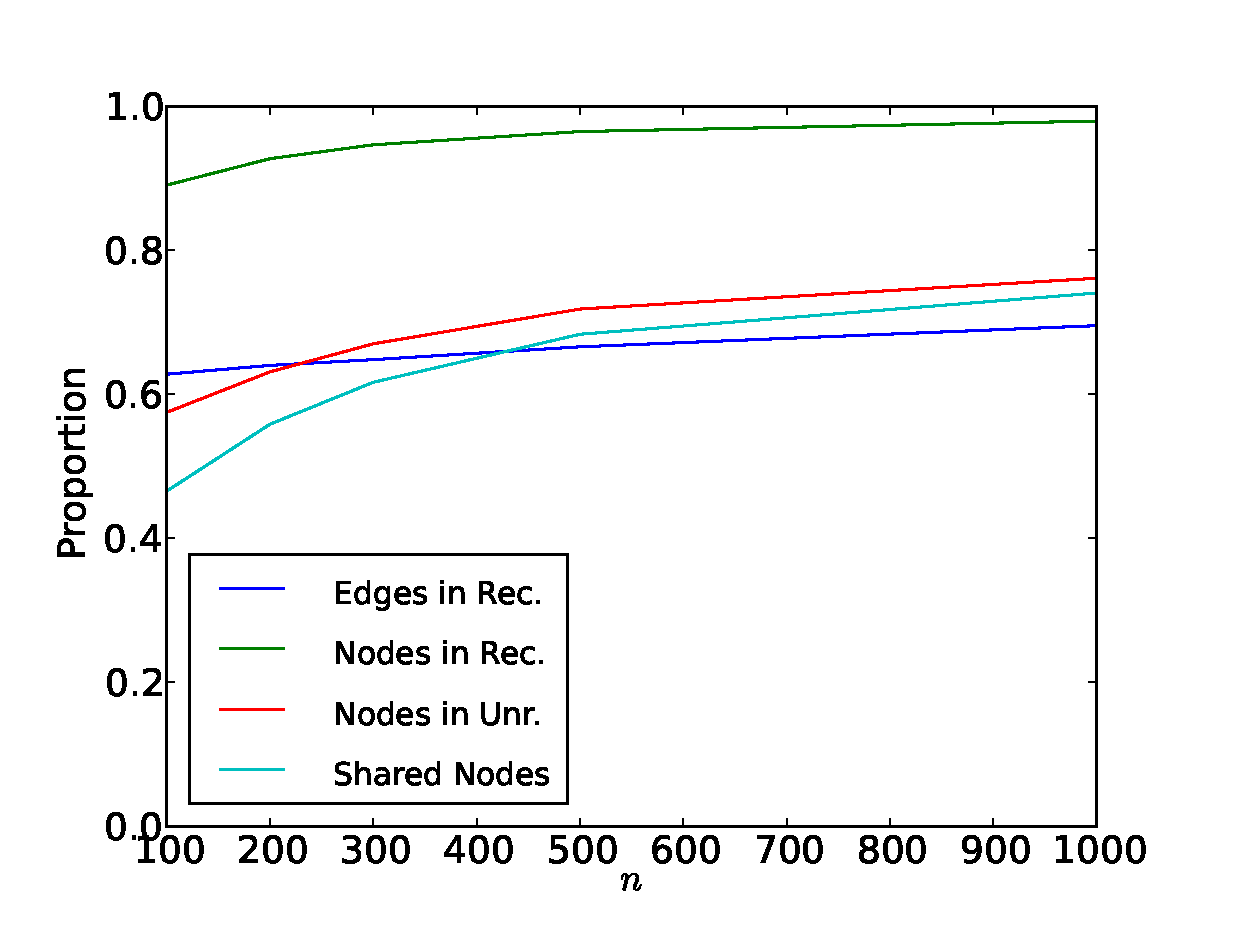
\includegraphics[width=2.5in]{proportion_edgesnodes_n}                
\caption{Proportion of nodes or edges (varying $n$)}
\label{fig_rur_propn}
\end{figure}

\begin{figure}[!t]
\centering
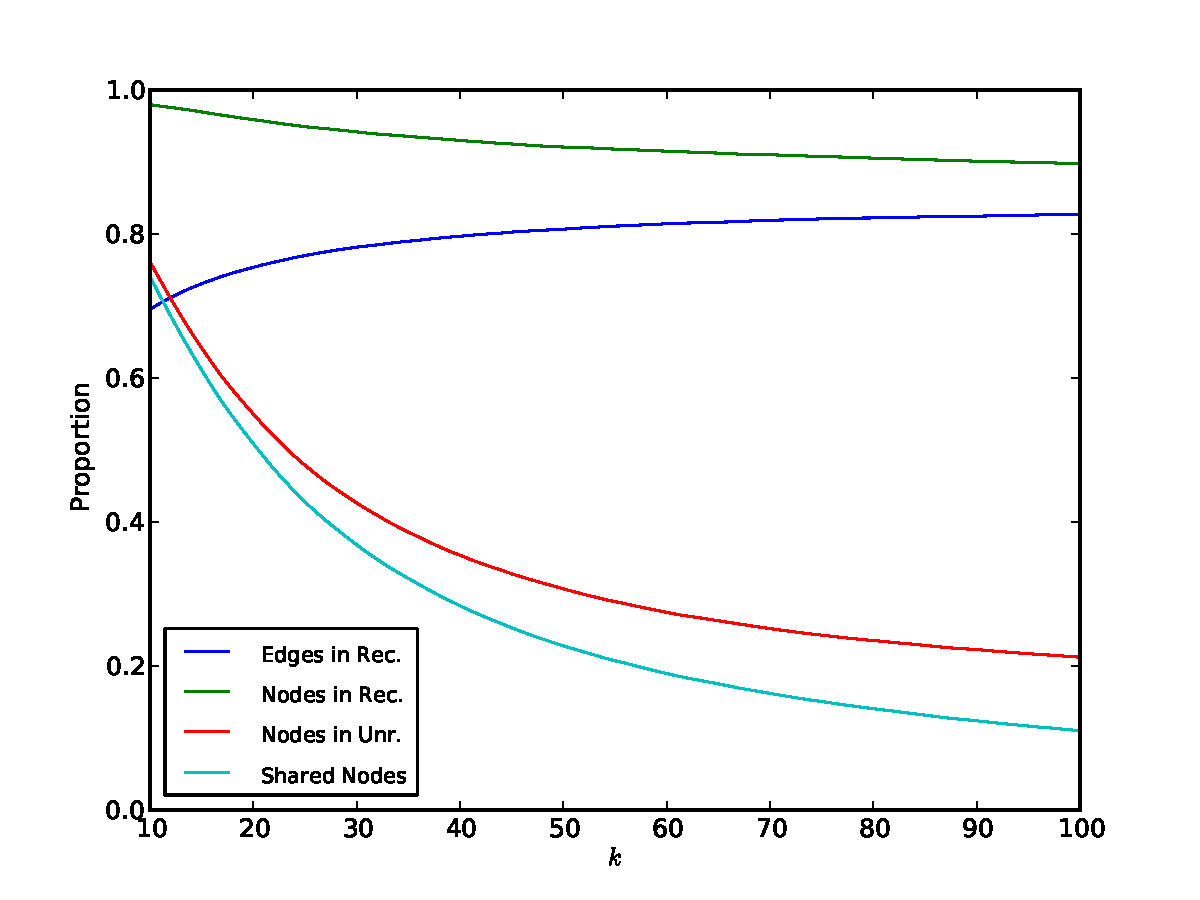
\includegraphics[width=2.5in]{proportion_edgesnodes_k}                
\caption{Proportion of nodes or edges (varying $k$)}
\label{fig_rur_propk}
\end{figure}

\begin{figure}[!t]
\centering
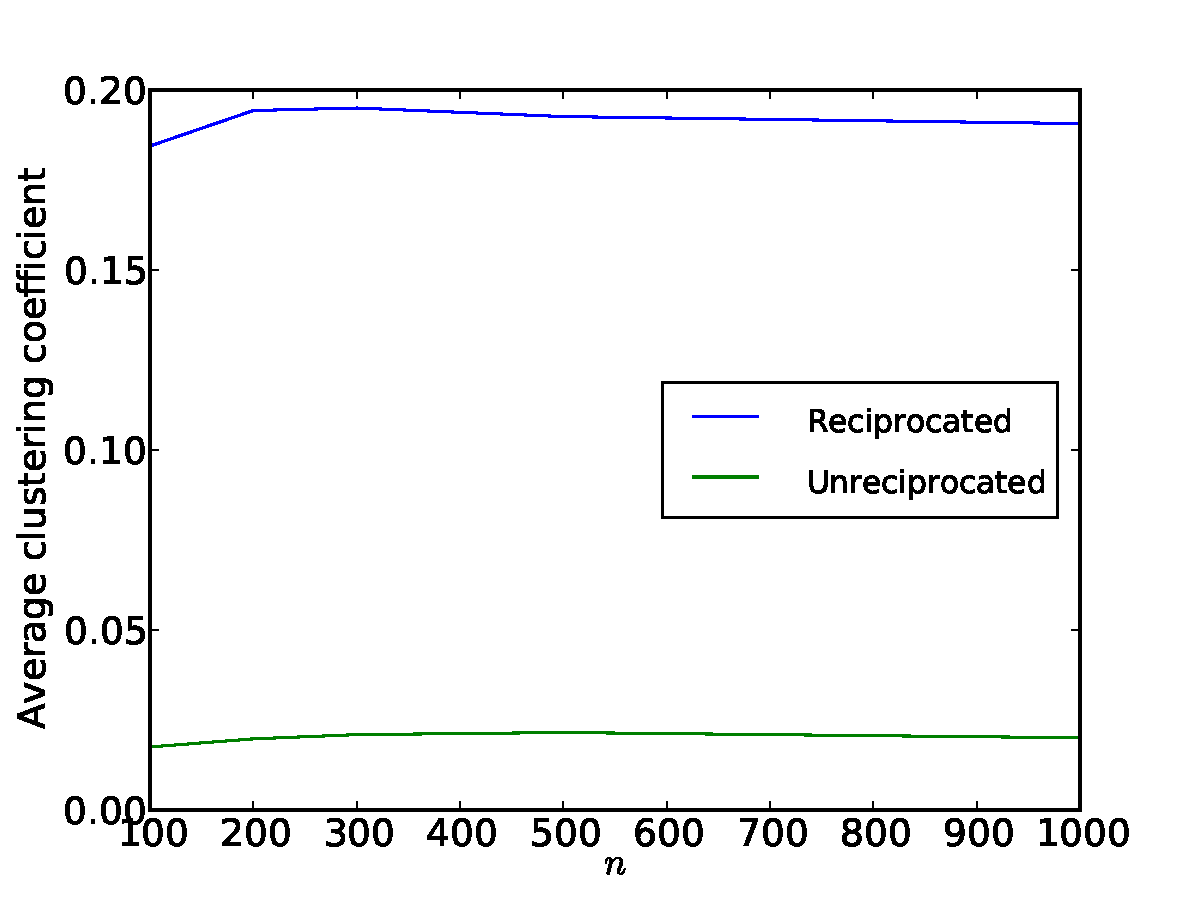
\includegraphics[width=2.5in]{average_clustering_n}          
\caption{Clustering coefficient (varying $n$)}
\label{fig_rur_cc_n}
\end{figure}

\begin{figure}[!t]
\centering
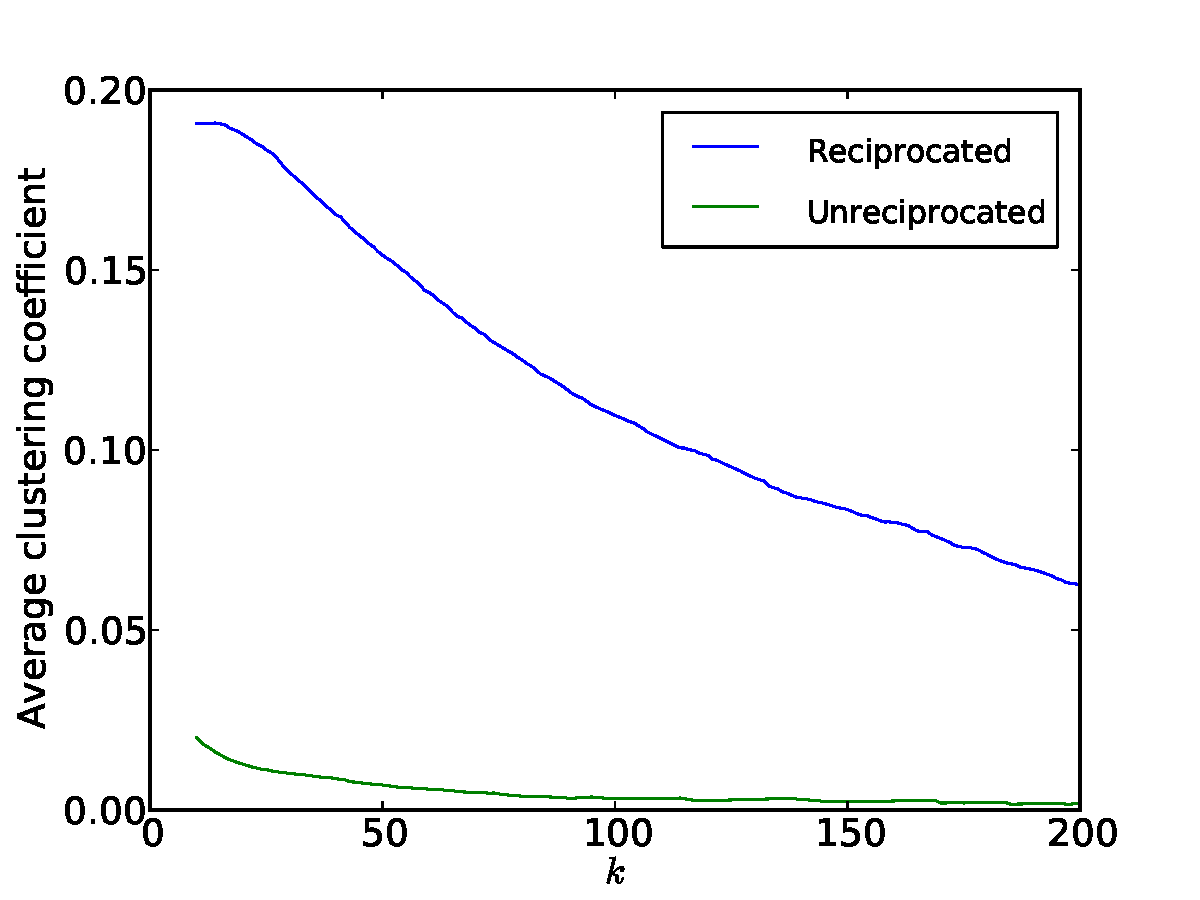
\includegraphics[width=2.5in]{average_clustering_k}      
\caption{Clustering coefficient (varying $k$)}
\label{fig_rur_cc_k}
\end{figure}

\begin{figure}[!t]
\centering
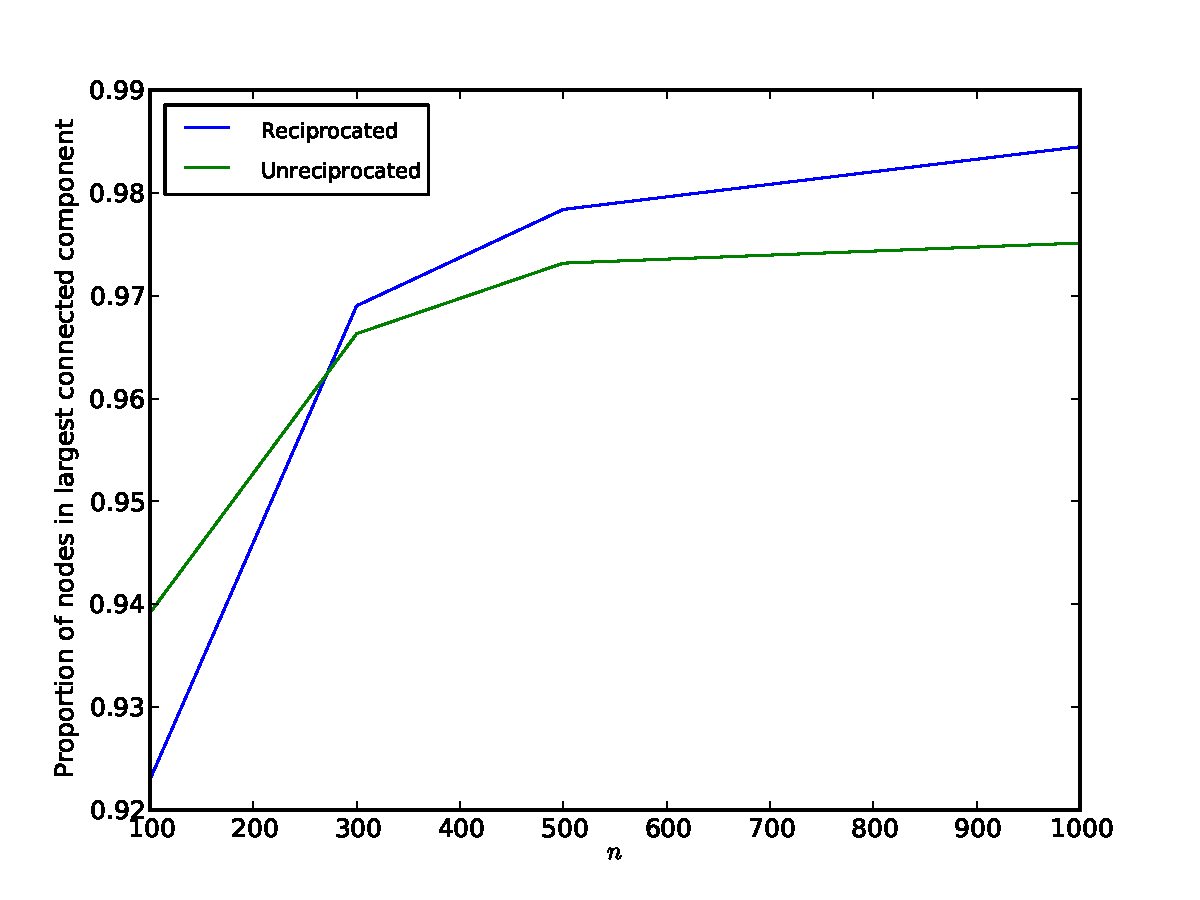
\includegraphics[width=2.5in]{proportion_largestcc_n}
\caption{Proportion in largest connected component (varying $n$)}
\label{fig_rur_lcc_n}
\end{figure}

\begin{figure}[!t]
\centering
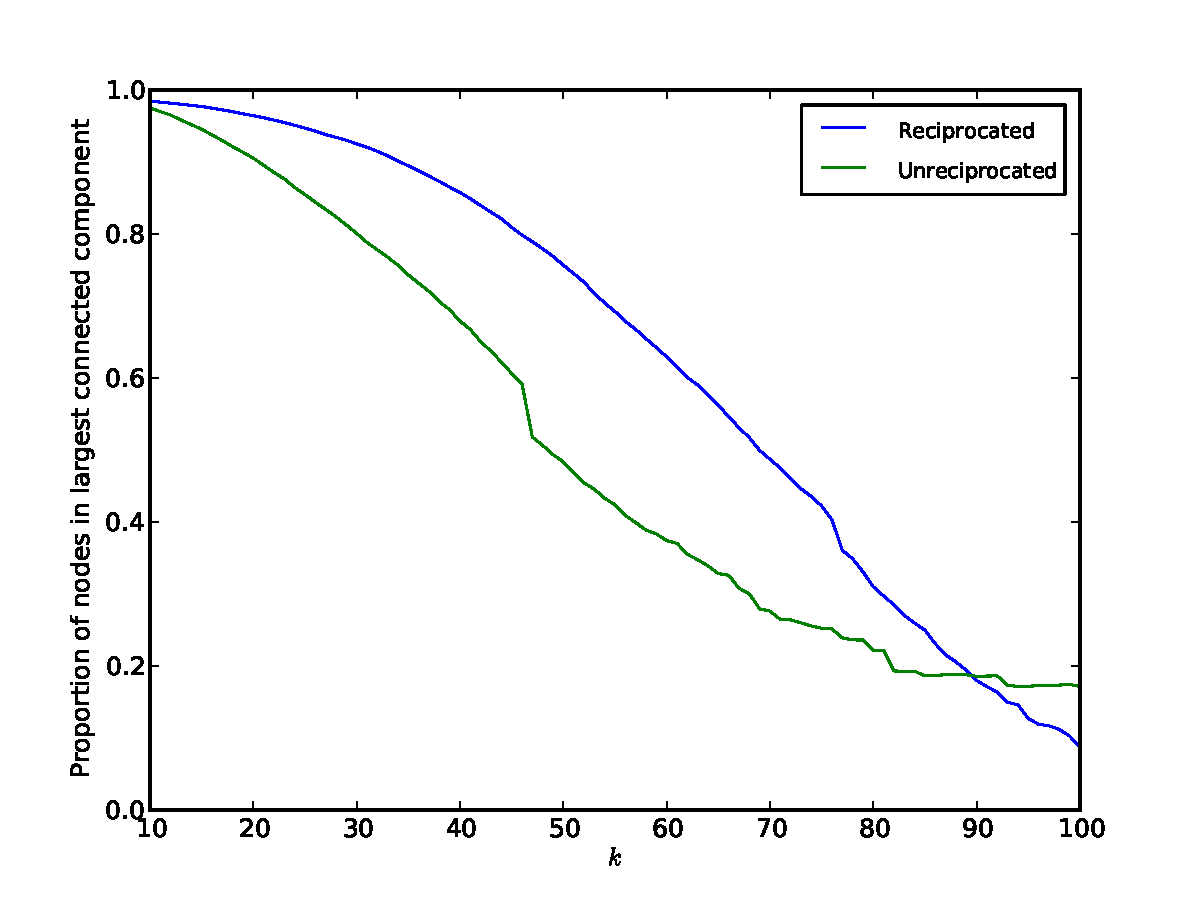
\includegraphics[width=2.5in]{proportion_largestcc_k}
\caption{Proportion in largest connected component (varying $k$)}
\label{fig_rur_lcc_k}
\end{figure}

%\begin{figure}[!t]
%\centering
%\subfloat[Varying $n$]{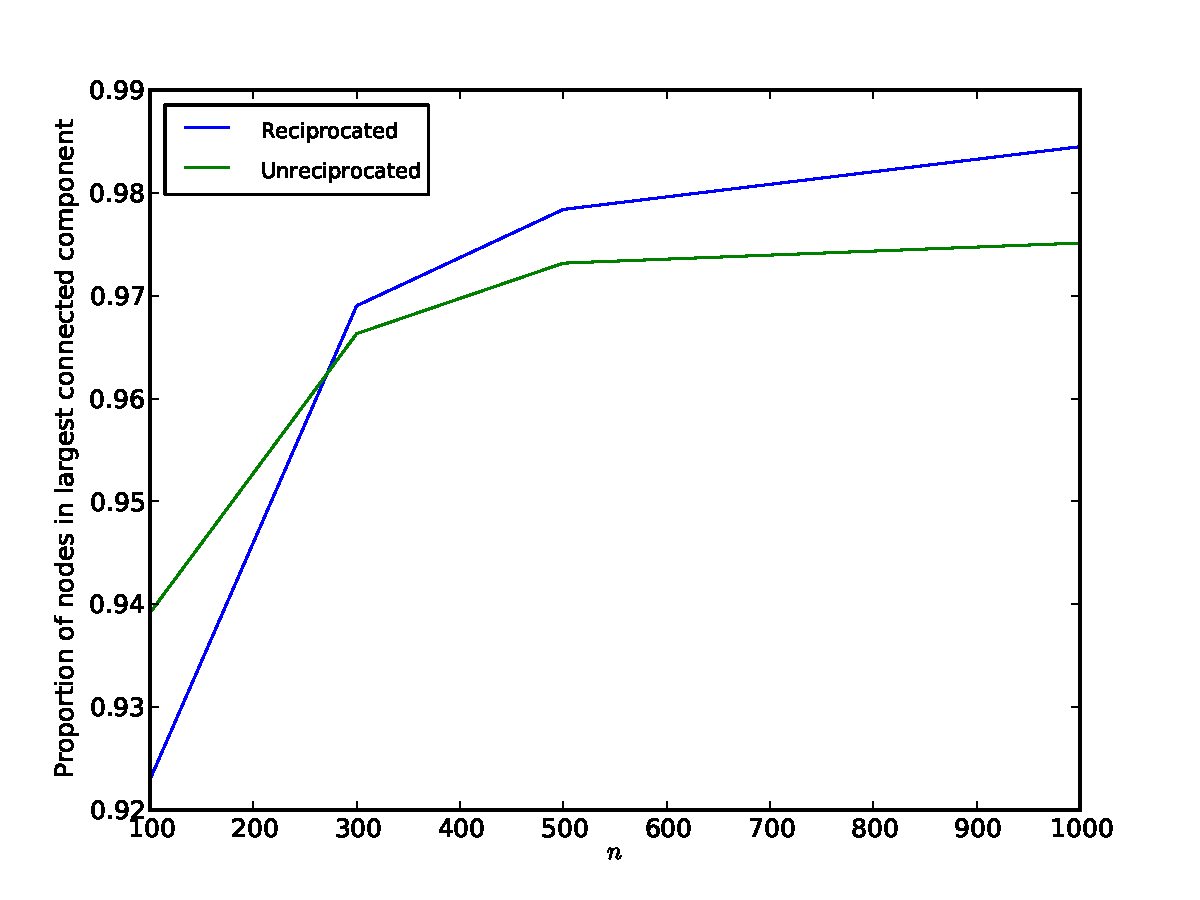
\includegraphics[width=1.5in]{proportion_largestcc_n}}                
%\subfloat[Varying $k$]{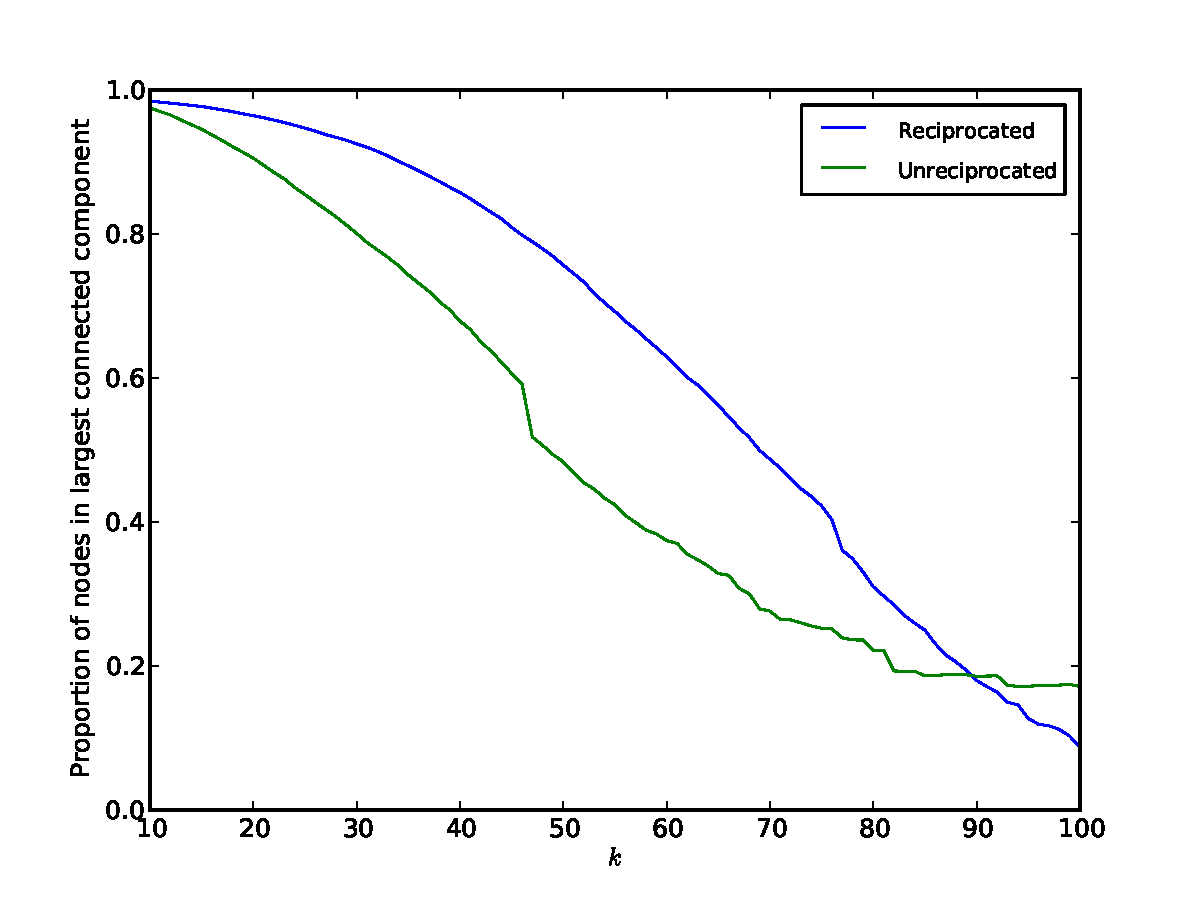
\includegraphics[width=1.5in]{proportion_largestcc_k}}
%\caption{Proportion in largest connected component}
%\label{fig_rur_lcc}
%\end{figure}

\begin{figure}[!t]
\centering
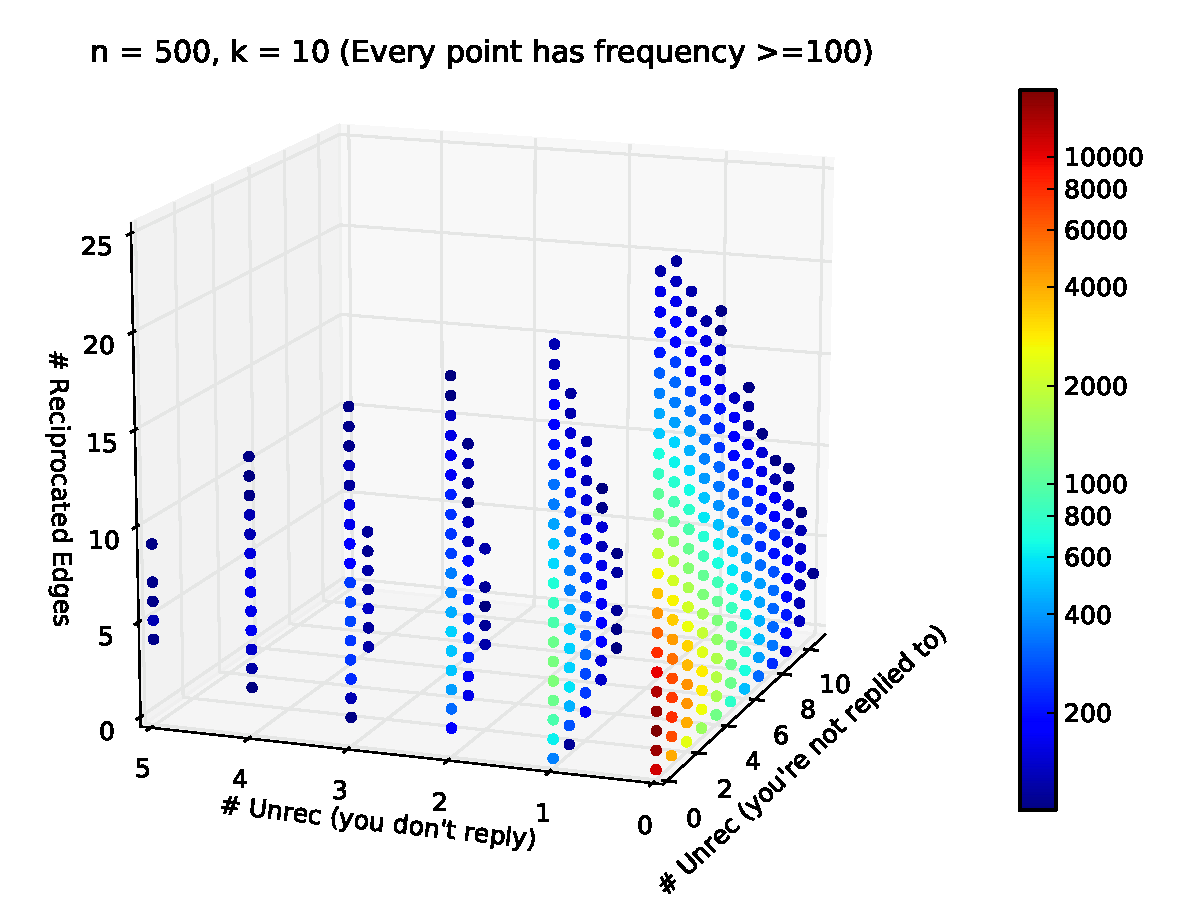
\includegraphics[width=2.5in]{scatter3}
\caption{Scatter plot of users' interaction types}
\label{fig_rur_sca2}
\end{figure}

% An example of a double column floating figure using two subfigures.
% (The subfig.sty package must be loaded for this to work.)
% The subfigure \label commands are set within each subfloat command, the
% \label for the overall figure must come after \caption.
% \hfil must be used as a separator to get equal spacing.
% The subfigure.sty package works much the same way, except \subfigure is
% used instead of \subfloat.
%
%\begin{figure*}[!t]
%\centerline{\subfloat[Case I]\includegraphics[width=2.5in]{subfigcase1}%
%\label{fig_first_case}}
%\hfil
%\subfloat[Case II]{\includegraphics[width=2.5in]{subfigcase2}%
%\label{fig_second_case}}}
%\caption{Simulation results}
%\label{fig_sim}
%\end{figure*}
%
% Note that often IEEE papers with subfigures do not employ subfigure
% captions (using the optional argument to \subfloat), but instead will
% reference/describe all of them (a), (b), etc., within the main caption.

\section{Conclusion}
To be written.


\section*{Acknowledgment}
 This work was supported by (SOMEGRANT).


\bibliographystyle{IEEEtran}
\bibliography{rec}

\end{document}


